%
% stackleer.tex
%
% (c) 2019 Prof Dr Andreas Müller, Hochschule Rapperswil
%
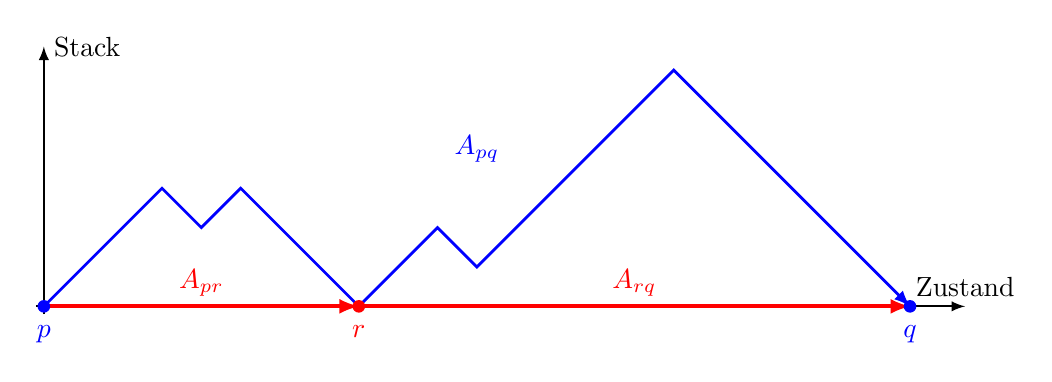
\begin{tikzpicture}[>=latex,thick]

\draw[->,line width=0.7pt] (-0.1,0)--(11.7,0) coordinate[label={Zustand}];
\draw[->,line width=0.7pt] (0,-0.1)--(0,3.3) coordinate[label={right:Stack}];

\draw[->,line width=1pt,color=blue]
	  ( 0.0,0.0)
	--( 1.5,1.5)
	--( 2.0,1.0)
	--( 2.5,1.5)
	--( 4.0,0.0)
	--( 5.0,1.0)
	--( 5.5,0.5)
	--( 8.0,3.0)
	--(11.0,0.0);

\fill[color=red] ( 4.0,0.0) circle[radius=0.08];
\node[color=red] at ( 4.0,0.0) [below] {$\mathstrut r$};

\draw[->,line width=1.4pt,color=red] (0,0)--(4.0,0);
\draw[->,line width=1.4pt,color=red] (4.0,0)--(11.0,0);
\node[color=red] at (2,0) [above] {$A_{pr}$};
\node[color=red] at (7.5,0) [above] {$A_{rq}$};

\node[color=blue] at (5.5,2) {$A_{pq}$};

\fill[color=blue] ( 0.0,0.0) circle[radius=0.08];
\fill[color=blue] (11.0,0.0) circle[radius=0.08];

\node[color=blue] at ( 0.0,0.0) [below] {$\mathstrut p$};
\node[color=blue] at (11.0,0.0) [below] {$\mathstrut q$};

\end{tikzpicture}
